% Sequence diagrams of the three subscriber-side track-switching methods
% compared in "Zero Gap, Zero Waste: Subscriber-Initiated, Relay-Executed
% Track Switching in MOQ Transport" (IEEE MMSP 2026).
%
% These were cut from the paper for space. Build a standalone PDF with:
%     pdflatex switching-methods.tex
%
\documentclass[border=6pt]{standalone}
\usepackage{tikz}
\usepackage{xspace}
\newcommand{\boxtext}[1]{\texttt{#1}}
\newcommand{\subm}{\boxtext{SUBSCRIBE}\xspace}
\newcommand{\subok}{\boxtext{SUBSCRIBE\_OK}\xspace}
\newcommand{\fetchm}{\boxtext{FETCH}\xspace}
\newcommand{\joiningfetch}{Joining~\fetchm}
\newcommand{\requpdate}{\boxtext{REQUEST\_UPDATE}\xspace}
\newcommand{\switchm}{\boxtext{SWITCH}\xspace}
\begin{document}
\begin{tabular}{@{}c@{}}
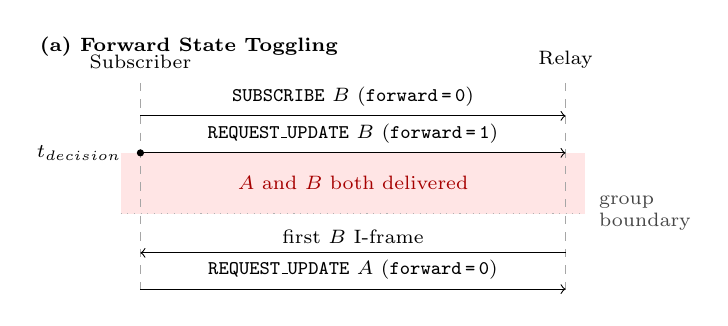
\begin{tikzpicture}[font=\scriptsize,x=1cm,y=1cm]
  \node[anchor=west,font=\scriptsize\bfseries] at (0,0.40) {(a) Forward State Toggling};
  \fill[red!10] (1.15,-1.72) rectangle (7.05,-0.95);
  \node[anchor=south] at (1.40,0.00) {Subscriber};
  \node[anchor=south] at (6.80,0.00) {Relay};
  \draw[gray!70,dashed] (1.40,-0.06) -- (1.40,-2.78);
  \draw[gray!70,dashed] (6.80,-0.06) -- (6.80,-2.78);
  \draw[->] (1.40,-0.48) -- node[above]{\subm $B$ (\texttt{forward\,=\,0})} (6.80,-0.48);
  \fill (1.40,-0.95) circle (1.3pt);
  \node[anchor=east] at (1.28,-0.95) {$t_{decision}$};
  \draw[->] (1.40,-0.95) -- node[above]{\requpdate $B$ (\texttt{forward\,=\,1})} (6.80,-0.95);
  \node[red!65!black] at (4.10,-1.33) {$A$ and $B$ both delivered};
  \draw[gray!60,dotted] (1.15,-1.72) -- (7.05,-1.72);
  \node[anchor=west,gray!55!black,align=left] at (7.10,-1.72) {group\\boundary};
  \draw[->] (6.80,-2.22) -- node[above]{first $B$ I-frame} (1.40,-2.22);
  \draw[->] (1.40,-2.68) -- node[above]{\requpdate $A$ (\texttt{forward\,=\,0})} (6.80,-2.68);
\end{tikzpicture}

\vspace{8pt}

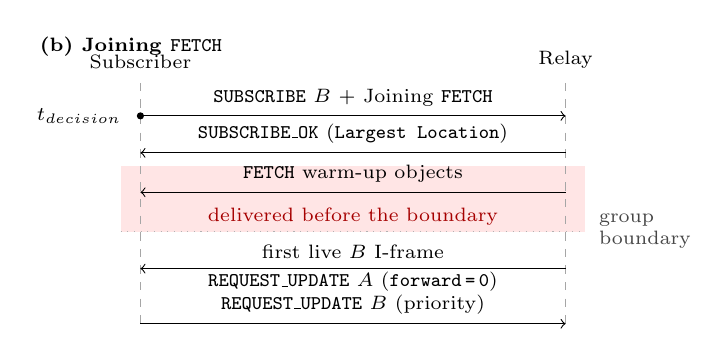
\begin{tikzpicture}[font=\scriptsize,x=1cm,y=1cm]
  \node[anchor=west,font=\scriptsize\bfseries] at (0,0.40) {(b) \joiningfetch};
  \fill[red!10] (1.15,-1.95) rectangle (7.05,-1.12);
  \node[anchor=south] at (1.40,0.00) {Subscriber};
  \node[anchor=south] at (6.80,0.00) {Relay};
  \draw[gray!70,dashed] (1.40,-0.06) -- (1.40,-3.22);
  \draw[gray!70,dashed] (6.80,-0.06) -- (6.80,-3.22);
  \fill (1.40,-0.48) circle (1.3pt);
  \node[anchor=east] at (1.28,-0.48) {$t_{decision}$};
  \draw[->] (1.40,-0.48) -- node[above]{\subm $B$ $+$ \joiningfetch} (6.80,-0.48);
  \draw[->] (6.80,-0.95) -- node[above]{\subok (\texttt{Largest Location})} (1.40,-0.95);
  \draw[->] (6.80,-1.45) -- node[above]{\fetchm warm-up objects} (1.40,-1.45);
  \node[red!65!black] at (4.10,-1.76) {delivered before the boundary};
  \draw[gray!60,dotted] (1.15,-1.95) -- (7.05,-1.95);
  \node[anchor=west,gray!55!black,align=left] at (7.10,-1.95) {group\\boundary};
  \draw[->] (6.80,-2.42) -- node[above]{first live $B$ I-frame} (1.40,-2.42);
  \draw[->] (1.40,-3.12) -- node[above,align=center]{\requpdate $A$ (\texttt{forward\,=\,0})\\\requpdate $B$ (priority)} (6.80,-3.12);
\end{tikzpicture}

\vspace{8pt}

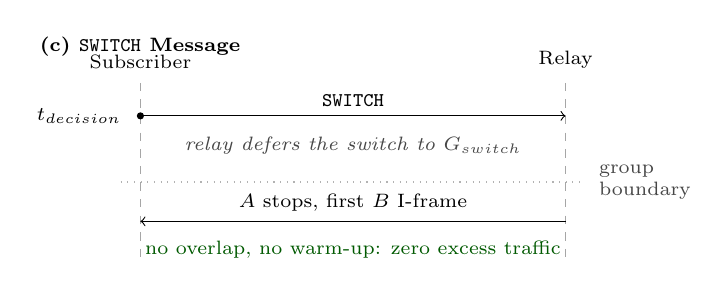
\begin{tikzpicture}[font=\scriptsize,x=1cm,y=1cm]
  \node[anchor=west,font=\scriptsize\bfseries] at (0,0.40) {(c) \switchm Message};
  \node[anchor=south] at (1.40,0.00) {Subscriber};
  \node[anchor=south] at (6.80,0.00) {Relay};
  \draw[gray!70,dashed] (1.40,-0.06) -- (1.40,-2.28);
  \draw[gray!70,dashed] (6.80,-0.06) -- (6.80,-2.28);
  \fill (1.40,-0.48) circle (1.3pt);
  \node[anchor=east] at (1.28,-0.48) {$t_{decision}$};
  \draw[->] (1.40,-0.48) -- node[above]{\switchm} (6.80,-0.48);
  \node[gray!55!black,font=\scriptsize\itshape] at (4.10,-0.86) {relay defers the switch to $G_{switch}$};
  \draw[gray!60,dotted] (1.15,-1.32) -- (7.05,-1.32);
  \node[anchor=west,gray!55!black,align=left] at (7.10,-1.32) {group\\boundary};
  \draw[->] (6.80,-1.82) -- node[above]{$A$ stops, first $B$ I-frame} (1.40,-1.82);
  \node[green!35!black] at (4.10,-2.18) {no overlap, no warm-up: zero excess traffic};
\end{tikzpicture}
\end{tabular}
\end{document}
